% Title page
\frame[plain]{\titlepage}

% Lesson 1. Introduction, main terms and simple examples
\lecture{Intro}{intro}

\section{Tools}

\begin{frame}
	\frametitle{\insertsection}
	We are going to use SWI-Prolog~--- a comprehensive free Prolog environment.
	\begin{itemize}
		\item You can download SWI-Prolog at this page: \href{https://www.swi-prolog.org/download/stable}{https://www.swi-prolog.org/download/stable}
		\item Complete manual is available at \href{https://www.swi-prolog.org/pldoc/doc_for?object=manual}{https://www.swi-prolog.org/pldoc/doc\_for?object=manual}
		\item Online tool SWISH: \href{https://swish.swi-prolog.org/}{https://swish.swi-prolog.org/}
		\item Eclipse PDT~--- Prolog Development Tool
	\end{itemize}
\end{frame}

\section{Overview}

\begin{frame}
	\frametitle{\insertsection}
	Goals of the lesson
	\begin{itemize}
		\item Look into the syntax of Prolog language
		\item Define the main terms of Prolog: fact, rule, query, and knowledge base
		\item Define basic syntax units, such as atom, variables and term
		\item Look at some example programs and try to figure out what they do
		\item Get out feet wet with some programming
	\end{itemize}
\end{frame}

\section{Basic constructs}

\begin{frame}
	\frametitle{\insertsection}
	Basic Prolog constructs
	\begin{tabular}{p{0.4\textwidth}p{.6\textwidth}}
		\begin{itemize}
			\item \textbf{Facts}. Facts are used to state things that are unconditionally true in the domain of interest.
			\item \textbf{Rules}. Rules state information that is conditionally true of the domain of interest.
		\end{itemize}
		&
		\begin{itemize}
			\item[] \textbf{Knowledge Base} (also called database) is a collection of facts and rules. Prolog programs are knowledge
			bases, collections of facts and rules which describe some collection of relationships that we find interesting. We use knowledge base
			by posing queries.
		\end{itemize}
	\end{tabular}
	\begin{itemize}
		\item \textbf{Queries}. The Prolog interpreter responds to queries about the facts and rules represented in its database. In making a query you are asking Prolog whether it can prove that your query is true. If so, it answers "Yes" and displays any \textit{variable bindings} that it made in coming up with the answer. If it fails to prove the query true, it answers "No".
	\end{itemize}
\end{frame}

\section{Simple Examples}

\begin{frame}
	\frametitle{\insertsection}
	\textbf{Example 1}: Simple knowledge base
	
	\begin{tabular}{p{0.4\textwidth}|l}
			\textbf{Knowledge base} & \only<2->{\textbf{Possible queries and responses}} \\
			\hline
			\hline
			\texttt{
				\begin{tabular}{p{0.5\textwidth}}
					fruit(orange).\\
					fruit(apple).\\
					vegetable(potato).\\
					vegetable(onion).\\
					\only<3->{common(you).\\
						uncommon(chuck\_norris).\\
						makes\_cry(onion, Person) :- common(Person).\\
						makes\_cry(Person, onion) :- uncommon(Person).\\
					}
				\end{tabular}
			} &
			\texttt{\only<2>{\begin{tabular}{l l}
				?- fruit(orange). & \textbf{true.} \\
				\hline
				?- fruit(onion). & \textbf{false.} \\
				\hline
				?- fruit(tomato). & \textbf{false.} \\
				\hline
				?- berry(watermelon). & \textbf{ERROR}
			\end{tabular}} \only<4->{\begin{tabular}{p{0.3\textwidth}p{0.2\textwidth}}
				?- makes\_cry(chuck\_norris, onion). & \textbf{true.} \\
				\hline
				?- makes\_cry(onion, you). & \textbf{true.} \\
				\hline
				?- makes\_cry(you, onion). & \textbf{false.} \\
				\hline
				?- makes\_cry(Who, Whom). & Who=you, \newline  Whom=onion; \newline  Who=chuck\_norris, \newline  Whom=onion. \\
		\end{tabular}}}
	\end{tabular}
\end{frame}

\begin{frame}
	\frametitle{\insertsection}
	\textbf{Example 2}: Conjunctions and disjunctions in rules
	
	\begin{tabular}{p{0.5\textwidth}|l}
		\textbf{Knowledge base} & \only<2->{\textbf{Possible queries and responses}} \\
		\hline
		\hline
		\texttt{
			\begin{tabular}{p{0.5\textwidth}}
				lovesMusic(anna).\\
				lovesMusic(sam).\\
				playsInstrument(anna).\\
				musician(P) :- lovesMusic(P),\newline playsInstrument(P).\\
				melomaniac(P) :- !,lovesMusic(P);\newline playsInstrument(P).\\
			\end{tabular}
		} &
		\texttt{\only<2->{\begin{tabular}{p{0.3\textwidth}p{0.2\textwidth}}
					?- musician(anna) & \textbf{true.} \\
					\hline
					?- musician(sam) & \textbf{false.} \\
					\hline
					?- melomaniac(anna) & \textbf{true.} \\
					\hline
					?- melomaniac(sam) & \textbf{true.} \\
					\hline
					?- melomaniac(Person) & \textbf{Person=sam; Person=anna.}
			\end{tabular}}}
	\end{tabular}
\end{frame}

\begin{frame}
	\frametitle{\insertsection}
	\textbf{Example 3}: Negations
	
	\begin{tabular}{p{0.5\textwidth}|l}
		\textbf{Knowledge base} & \only<2->{\textbf{Possible queries and responses}} \\
		\hline
		\hline
		\texttt{
			\begin{tabular}{p{0.5\textwidth}}
				cat(fluffy).\\
				cat(cornie).\\
				bird(butch).\\
				dog(bayley).\\
				good(fluffy).\\
				hasClaws(X) :- cat(X).\\
				hasClaws(X) :- bird(X).\\
				hasClaws(X) :- not(dog(X)).\\
				animal(X) :- cat(X);bird(X);dog(X).\\
				domestic(X) :- animal(X),not(hasClaws(X)).\\
				domestic(X) :- animal(X),good(X).\\
			\end{tabular}
		} &
		\texttt{\only<2->{\begin{tabular}{p{0.3\textwidth}p{0.2\textwidth}}
					?- domestic(bayley). & \textbf{true.} \\
					\hline
					?- domestic(cornie). & \textbf{false.} \\
					\hline
					?- cat(C),domestic(C) & \textbf{C = fluffy.}\\
					\hline
					?- cat(C),not(domestic(C)) & \textbf{C = cornie.}
		\end{tabular}}}
	\end{tabular}
\end{frame}

\section{Prolog Syntax}

\begin{frame}
	\frametitle{\insertsection}
	\textbf{Facts, rules and queries in Prolog are built of terms}
	\begin{itemize}
		\item Atoms
		\item Numbers
		\item Strings
		\item Variables
		\item Compex terms~--- structures
	\end{itemize}
\end{frame}

\begin{frame}
	\frametitle{\insertsection}
	\textbf{Atoms}
	\begin{enumerate}
		\item A string of characters made up of upper-case letters, lower-case letters, digits, and underscore characters,
		that begins with a lower-case letter.
		\item An arbitrary sequence of characters enclosed in single quotes.
		\item A sequence of special characters.
	\end{enumerate}

	\begin{example}
		\texttt{chuck\_norris, bayley, cornie, someCamelCaseStringNumber1, 'Chuck Norris', 'Some arbitrary string', '@!?@',
		=====>, :-, @>}
	\end{example}
\end{frame}

\begin{frame}
	\frametitle{\insertsection}
	\textbf{Numbers}
	\begin{enumerate}
		\item \textbf{Real numbers}, though not particularly important in typical applications, are supported in Prolog.
		\item[] \begin{example}
			2.71828, 82.19284, \(\pi, e \), \ldots
		\end{example}
		\item \textbf{Integers} are useful for many tasks, such as counting the elements of a list.
		\item[] \begin{example}
			\(-2, -1, 0, 1, 2, 3, \ldots \)
		\end{example}
	\end{enumerate}
\end{frame}

\begin{frame}
	\frametitle{\insertsection}
	\textbf{Variables and strings}
	\begin{enumerate}
		\item A variable is a sequence of upper-case letters, lower-case letters, digits and underscore character
		that starts either with an upper-case letter or with underscore.
		\item[] \begin{example}
			\texttt{X, Y, Var, Chuck\_Norris, \_someVar, \_1zx, \_}
		\end{example}
		\item String is an arbitrary sequence of characters enclosed in double quotes.
		\item[] \begin{example}
			"Some arbitrary string line"
		\end{example}
	\end{enumerate}
\end{frame}

\begin{frame}
	\frametitle{\insertsection}
	\textbf{Complex terms}
	\only<1>{\begin{itemize}
		\item Complex terms are built out of \textbf{functor (predicate)} followed by a sequence of \textbf{arguments}.
		\item The arguments are put in parentheses and are separated by commas.
		\item The functor of a term \textbf{must} be an atom.
		\item Arguments can be any kind of term.
		\item The number of arguments that a complex term has is called its \textbf{arity}.
	\end{itemize}}
	\only<2->{\begin{itemize}
			\item Any \textbf{constant} is a term. Constants are atoms, numbers or strings.
			\item Any \textbf{variable} is a term.
			\item Any sequence of a form \texttt{f(a1, a2, \ldots)} where \texttt{f} is an atom, and
			\texttt{a1, a2,}~\ldots are terms, is a term.
			\item There are no other terms.
	\end{itemize}
	\begin{example}
		\texttt{g(f(x, y))}
	\end{example}}
	
\end{frame}

\begin{frame}
	\frametitle{\insertsection}
	Which of the character sequences are atoms, variables or neither of them?
	\texttt{\begin{enumerate}
		\item vARIABLE
		\item Variable
		\item x
		\item XY1
		\item chuck\_norris\_tells\_simon\_what\_to\_do
		\item \_john
		\item '\_jonh'
		\item 'John likes everybody'
		\item Chuck Norris plays russian roulette with a fully loded revolver and wins
	\end{enumerate}}
\end{frame}

\begin{frame}
	\frametitle{\insertsection}
	Which of the sequences are terms, and which are not. For every term indicate its functor and arity.
	\texttt{\begin{enumerate}
		\item loves(vincent,mia)
		\item 'loves(vincent,mia)'
		\item Eats(cat,mouse)
		\item hasChildren(cat,kittens)
		\item and(musician(jody),artist(mia))
		\item and(musician(X),artist(Y))
		\item \_and(musician(jody),artist(mia))
		\item (Butch kills Vincent)
		\item kills(Butch,Vincent)
	\end{enumerate}}
\end{frame}

\begin{frame}
	\frametitle{\insertsection}
	How many facts, rules, clauses and predicates there are in the knowledge base?
	
	\texttt{
		\begin{tabular}{l}
			cat(fluffy).\\
			cat(cornie).\\
			bird(butch).\\
			dog(bayley).\\
			good(fluffy).\\
			hasClaws(X) :- cat(X).\\
			hasClaws(X) :- bird(X).\\
			hasClaws(X) :- not(dog(X)).\\
			animal(X) :- cat(X);bird(X);dog(X).\\
			domestic(X) :- animal(X),not(hasClaws(X)).\\
			domestic(X) :- animal(X),good(X).\\
		\end{tabular}
	}
\end{frame}

\section{Exercise}

\begin{frame}
	\frametitle{\insertsection}
	\textbf{Write the following statements in Prolog}
	
	\texttt{\begin{tabular}{l}
			1. Any giraffe is a horse that was uppercutted by Chuck Norris \\
			2. Mia and Marcellus are married \\
			3. Zed is dead \\
			4. If something is on fire then it smokes \\
			5. Marsellus kills everyone who gives Mia a footmassage \\
			6. Mother of a mother is a grandmother \\
			7. Mia loves everyone who is a good dancer
	\end{tabular}}
\end{frame}


% Lesson 2. Term matching.
\lecture{Match}{match}
%\setcounter{framenumber}{1}

\section{Overview}

\begin{frame}
	\frametitle{\insertsection}
	Goals of the lesson
	\begin{itemize}
		\item Discuss the idea of matching in Prolog.
		\item Explain the differences between Prolog matching and standard unification.
		\item Introduce the built-in predicate for matching.
		\item Explain the search strategy Prolog uses when trying to prove something.
	\end{itemize}
\end{frame}

\section{Matching}

\begin{frame}
	\frametitle{\insertsection}
	\begin{itemize}
		\item The basic idea of matching is follows: \textbf{Two terms match, if they are equal or if they contain variables that can be
			instantiated in such a way that the resulting terms are equal}.
		\item The built-in binary predicate \texttt{=/2} tests whether its two arguments match.
	\end{itemize}
	
	\textbf{The following terms match:}
	
	\texttt{
		\begin{tabular}{l}
			orange = orange. \\
			fruit(orange) = fruit(orange). \\
			cat(C) = cat(fluffy). \\
			cat(C) = cat(cornie). \\
			f(g(X,Y)) = f(g(x, Z)). \\
			f(g(X,Y)) = f(g(Z,y)). \\
			f(g(X,Y)) = f(g(a,b)).
		\end{tabular}
	}
\end{frame}

\begin{frame}
	\frametitle{\insertsection}
	\begin{enumerate}
		\item If \texttt{term1} and \texttt{term2} are constants, then \texttt{term1} and \texttt{term2} match if and only if they are the same atom, the same string or the same number.
		\item If \texttt{term1} is a variable and \texttt{term2} is any type of term, then \texttt{term1} and \texttt{term2} match, and \texttt{term1} is instantiated to \texttt{term2}. Vice versa is also true. If they are both variables, they’re both instantiated to each other, and we say that they \textbf{share values}.
		\item If \texttt{term1} and \texttt{term2} are complex terms, then they match if and only if:
		\begin{enumerate}
			\item They have the same functor and arity.
			\item All their corresponding arguments match.
			\item The variable instantiations are compatible.
		\end{enumerate}
		\item Two terms match if and only if it follows from the previous three clauses that they match.
	\end{enumerate}
\end{frame}

\begin{frame}
	\frametitle{\insertsection}
	\textbf{Let us have some examples:}
	
	\texttt{
		\begin{tabular}{p{0.8\textwidth} | l}
			chuckNorris = chuckNorris. & \textbf{true.} \\
			\hline
			100 = 100. & \textbf{true.} \\
			\hline
			chuckNorris = "chuckNorris". & \textbf{false.} \\
			\hline
			chuckNorris = 'chuckNorris'. & \textbf{true.} \\
			\hline
			100 = '100' & \textbf{false.} \\
			\hline
			Var1 = Var2 & \textbf{true.} \\
			\hline
			triang(p(1,1),p(Px,Py),p(Px1,8)) = triang(P,p(7,4),p(n(7),8)). & \textbf{true.} \\
			\hline
			triang(p(X,X),p(2,5),p(7,11)) = triang(p(1,7), P2, P3). & \textbf{false.} \\
			\hline
			f(X) = X. & \textbf{true?}
		\end{tabular}
	}
\end{frame}

\section{Unification}

\begin{frame}
	\frametitle{\insertsection}
	\begin{itemize}
		\item Terms are symbolic expressions used to model logical propositions.
		\item Terms can easily be represented as trees, where variables and constants are leaves and functors are branches.
		\item A substitution of terms is a set of variables paired with terms: \(\left\{(x_1\rightarrow t_1 ),\ldots, (x_n\rightarrow t_n ) \right\} \), where each pair represents a variable \(x_i\), that should be substituted with a term \(t_i\).
		\item \textbf{Unification} is the process of unifying equations, called terms, so that they become equivalent. This is done by finding a substitution which when applied on the variables of the terms will result in them becoming identical.
		\item A unification algorithm commonly takes 2 terms and returns this substitution if it exists. The substitution that unifies the terms is called \textbf{a unifier}.
	\end{itemize}
\end{frame}

\begin{frame}
	\frametitle{\insertsection}
	\begin{itemize}
		\item A unification algorithm performs \textbf{the occur check}.
		\item The occur check checks whether a variable appears among the arguments of the functor, which it is being unified with. This is required to prohibit infinite terms like \(X = f(X)\), which results in something like \(f(f(f(f(\ldots)))) \). This can create cycles that could cause termination problems.
	\end{itemize}

	Suppose we have the following terms. What will the Standard Unification Algorithm do?
	
	\begin{table}
		\centering
		\begin{tabular}{c}
			\(f(X_1, X_2, \ldots, X_n) \) \\
			\\
			\(f(g(X_0, X_0), g(X_1, X_1), \ldots, g(X_{n-1}, X_{n-1}) \)
		\end{tabular}
	\end{table}
\end{frame}

\begin{frame}
	\frametitle{\insertsection}
	\begin{table}
		\centering
		\begin{tabular}{c}
			\(f(X_1, X_2, \ldots, X_n) \) \\
			\\
			\(f(g(X_0, X_0), g(X_1, X_1), \ldots, g(X_{n-1}, X_{n-1}) \)
		\end{tabular}
	\end{table}
	\only<1>{
		\begin{itemize}
			\item Obviously enough, the algorithm will reduce the problem by recognizing that the two functors are identical.
			\item Then problem becomes to transform the variable input of the two functors such that they become identical. Hence the algorithm will start unifying the variables of \(f\).
			\item First \(X_1\) will be substituted with \(g(X_0, X_0)\). The rest of the list will then replace each instance of \(X_1\) with \(g(X_0, X_0)\).
			\item The latter means that \(X_2\) will be substituted with \(g(g(X_0, X_0), g(X_0, X_0)\) and so on.
		\end{itemize}
	}
	\only<2->{
		\begin{tabular}{l}
			\(X_1\rightarrow g(X_0, X_0) \) \\ \\
			\(X_2\rightarrow g(g(X_0, X_0), g(X_0, X_0)) \) \\ \\
			\(X_3\rightarrow g(g(g(X_0, X_0), g(X_0, X_0)), g(g(X_0, X_0), g(X_0, X_0)))  \) \\ \\
			\vdots \\ \\
			\(X_n\rightarrow g(g(g(g(g\ldots  \)
		\end{tabular}
	}
\end{frame}

\begin{frame}
	\frametitle{\insertsection}
	\begin{itemize}
		\item Prolog \textbf{omits} the occur check when matching terms since the running time of the occur check can escalate.
		\item Standard unification algorithms are \textbf{pessimistic}. They first look	for strange variables (using the occurs check) and only when they are sure that the two terms are "safe" do they go ahead and try and match them. So a standard unification algorithm will never get locked into a situation where it is endlessly trying to match two unmatchable terms.
		\item Prolog, on the other hand, is \textbf{optimistic}. It assumes that you are not going to give it anything dangerous. So it does not make an occurs check. As soon as you give it two terms, it charges full steam ahead and tries to match them.
	\end{itemize}
\end{frame}

\section{Proof search}

\begin{frame}
	\frametitle{\insertsection}
	Suppose we are working with the following knowledge base:
	
	\begin{tabular}{p{0.52\textwidth}|l}
		\texttt{
			\begin{tabular}{p{0.5\textwidth}}
				verb(drinks).\\
				noun(milk).\\
				noun(cat).\\
				article(a).\\
				subj(cat).\\
				obj(milk).\\ \\
				phrase(A,S,V,O) :- article(A), noun(S), subj(S), verb(V), noun(O), obj(O).\\ \\
			\end{tabular}
		} &
		\texttt{{
			\begin{tabular}{p{0.4\textwidth}}
				Suppose we then pose a query: \textbf{phrase(A,S,V,O).} \\ \\
				The answer will be \\ \\
				A = a, \\ S = cat, \\ V = drinks, \\ O = milk
			\end{tabular}
		}}
	\end{tabular}
\end{frame}

\begin{frame}
	\frametitle{\insertsection}
	\begin{figure}
		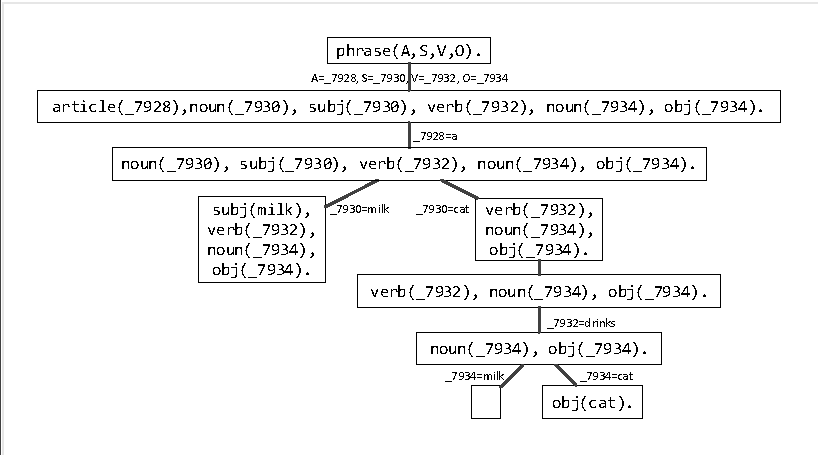
\includegraphics{prooftree}
	\end{figure}
\end{frame}

\section{Exercise}

\begin{frame}
	\frametitle{\insertsection}
	Which of the following pairs of terms match? Where relevant, give the variable instantiations that lead to successful matching.
	\texttt{\begin{enumerate}
		\item a = a, 'String' = string, x = Y.
		\item f(X, Y, z) = f(x, a, b).
		\item g(x, y, f(Z)) = g(Z, Y, f(x)).
		\item polygon(v(x1,y1), v(x1,Y), v(X,Y)) = polygon(v(X,Z), v(x1,y2), v(x3,y3)).
		\item polygon(v(x1,y3), v(x2,Y), v(X,Y)) = polygon(v(X,Y), v(Z,y3), v(x1,y3)).
		\item move(state(Pos,onTheFloor,Pos,H), push(Pos,Pos1), state(Pos1,onTheFloor,Pos1,H)) = move(state(x,onTheFloor,Pos,no), push(x,y), state(Pos1,onTheFloor,Pos1,no)).
	\end{enumerate}}
\end{frame}


% Lesson 3. Recursion in Prolog
\lecture{Recursion}{recursion}

\section{Overview}

\begin{frame}
	\frametitle{\insertsection}
	Goals of the lesson
	\begin{itemize}
		\item Introduce recursive definitions in Prolog
		\item Discuss the mismatches between the declarative meaning of a Prolog program, and its procedural meaning
	\end{itemize}
\end{frame}


\section{Recursive definitions}

\begin{frame}
	\frametitle{\insertsection}
	Predicates can be defined recursively. It means that one or more rules in predicate's definition refers to itself.
	
	\only<1>{The most common example is family relationships.}
	\only<2>{\textbf{Basis}}
	\only<3->{\textbf{Step}}
	
	\texttt{
		\begin{tabular}{l}
			{\color<2>[RGB]{255,0,0}{ancestor(Anc,Dec) :- child(Dec,Anc).}} \\
			{\color<3->[RGB]{255,0,0}{ancestor(Anc,Dec) :- child(Dec,Par), ancestor(Anc,Par).}} \\
			child(jane, peter). \\
			child(mary, kate). \\
			child(sam, mary). \\
			child(jason, jane). \\
			child(ann, jason).
		\end{tabular}
	}
\end{frame}


\begin{frame}
	\frametitle{\insertsection}
	
	Now, let us define natural numbers, having a definition of zero and a rule of succession.
	
	\texttt{
		\begin{tabular}{l}
			num(0). \\
			num(s(N)) :- num(N). \\ \\
			\uncover<2->{sum(0, N, N). \\
				sum(s(M), N, s(S)) :- sum(M, N, S).
			}
		\end{tabular}
	}

	\uncover<3->{Our numbers will be something like: \(0, s(0), s(s(0)), s(s(s(0))), \ldots\) Not very pleasant if you want to compute something, but sometimes used
	in automated provers.}
	
\end{frame}


\section{Tail recursion}

\begin{frame}
	\frametitle{\insertsection}
	
	Suppose we want to compute factorial (in normal numbers this time). We already know about recursion, and after a while will end up with a program similar to this one:
	
	\texttt{
		\begin{tabular}{l}
			f(0,1). \\
			f(N,F) :- N > 0, M is N - 1, f(M,Acc), F is Acc*N.
		\end{tabular}
	}

	Binary predicate \texttt{f/2} takes two arguments: natural number N and factorial of N. The table below shows possible queries.
	
	\texttt{\begin{table}\centering\begin{tabular}{l | l}
			f(4, F). & F = 24. \\
			\hline
			f(5, 120). & true. \\
			\hline
			f(X, 120). & ERROR \\
	\end{tabular}\end{table}}	
	
\end{frame}


\begin{frame}
	\frametitle{\insertsection}
	
	A recursive function is \textbf{tail recursive} when recursive call is the last thing executed by the function. It works in Prolog just well.
	Let us rewrite our factorial function, and make it tail recursive.
	
	\texttt{
		\begin{tabular}{l}
			f(N,N,F,F) :- !. \\
			f(N,M,Acc,F) :- M1 is M + 1, Acc1 is Acc * M1, f(N,M1,Acc1,F). \\
			factorial(N,F) :- f(N,1,1,F).
		\end{tabular}
	}

	As we can see predicate \texttt{f} takes 4 arguments now: natural number N, computation step M, result computed on step M, and total result F. Below are some examples.
	
	\texttt{\begin{table}\centering\begin{tabular}{l | l}
				factorial(4, F). & F = 24. \\
				\hline
				factorial(5, 120). & true. \\
				\hline
				factorial(X, 120). & X = 5. \\
	\end{tabular}\end{table}}	
	
\end{frame}


\section{Clause ordering, goal ordering, and termination}

\begin{frame}
	\frametitle{\insertsection}
	
	\only<1>{Recall our family program which as we know works just fine:}
	\only<2->{But what happens if we swap goals in the second rule?}
	
	\texttt{
		\begin{tabular}{l}
			ancestor(Anc,Dec) :- child(Dec,Anc). \\
			\only<1>{ancestor(Anc,Dec) :- child(Dec,Par), ancestor(Anc,Par).}
			\only<2->{\underline{ancestor(Anc,Dec) :- ancestor(Anc,Par), child(Dec,Par).}}\\
			child(jane, peter). \\
			child(mary, kate). \\
			child(sam, mary). \\
			child(jason, jane). \\
			child(ann, jason).
		\end{tabular}
	}

	\uncover<2->{If we pose query \texttt{ancestor(jane, ann)} we will get a correct answer (\texttt{true}), and then an error message which means that Prolog is looping. }

\end{frame}

\begin{frame}
	\frametitle{\insertsection}
	\begin{figure}
		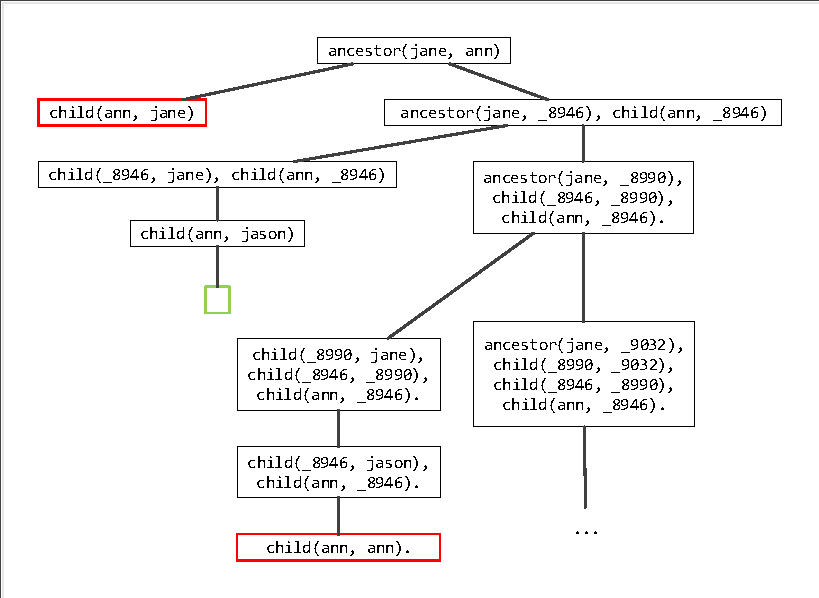
\includegraphics[scale=0.78]{badtree}
	\end{figure}
\end{frame}